\label{sec:cross-power}

In this section, I discuss how measurements of the 21\,cm and \lya\ fluctuation fields are
cross-correlated. To make a cross-correlation measurement of the 21\,cm and \lya\
fluctuation fields, I make use of the power spectrum, a statistical measurement
of the variance in fluctuations of some field at different spatial scales. The power
spectrum, $P \left({\bf k} \right)$, is formally defined using the following relationship,
\begin{equation}
\langle \widetilde{\delta}_i ({\bf k}) \widetilde{\delta}_j ({\bf k'}) \rangle = (2 \pi) ^3 \delta_D \left( {\bf k} - {\bf k'} \right) P_{ij} \left({\bf k} \right),
\end{equation}
where $\widetilde{\delta}$ is the Fourier transform of some fluctuation field, in this
case either 21\,cm or \lya, and $\delta_D$ is the Dirac delta function.
In practice, the power spectrum can be estimated with the relationship below
\begin{equation}
P_{ij}\left( k\right) \approx \frac{\sum_{\textbf{k} \in k} \widetilde{\delta}_i \left( \textbf{k}\right) \widetilde{\delta}_j \left( \textbf{k}\right)}{N_k V}
\end{equation}
where $N_k$ is the number of modes corresponding to a particular $k$ bin and $V$ is
the physical volume of survey. Instead of directly plotting, $P\left( k\right)$,
it is often common to scale the power spectrum to make its units independent of
scale,

\begin{equation}
    \widetilde{\Delta}^2_{ij} \left( k \right) = \frac{k^3}{2 \pi ^2} P_{ij} \left( k \right).
\end{equation}

\begin{figure}[ht]
	\centering
	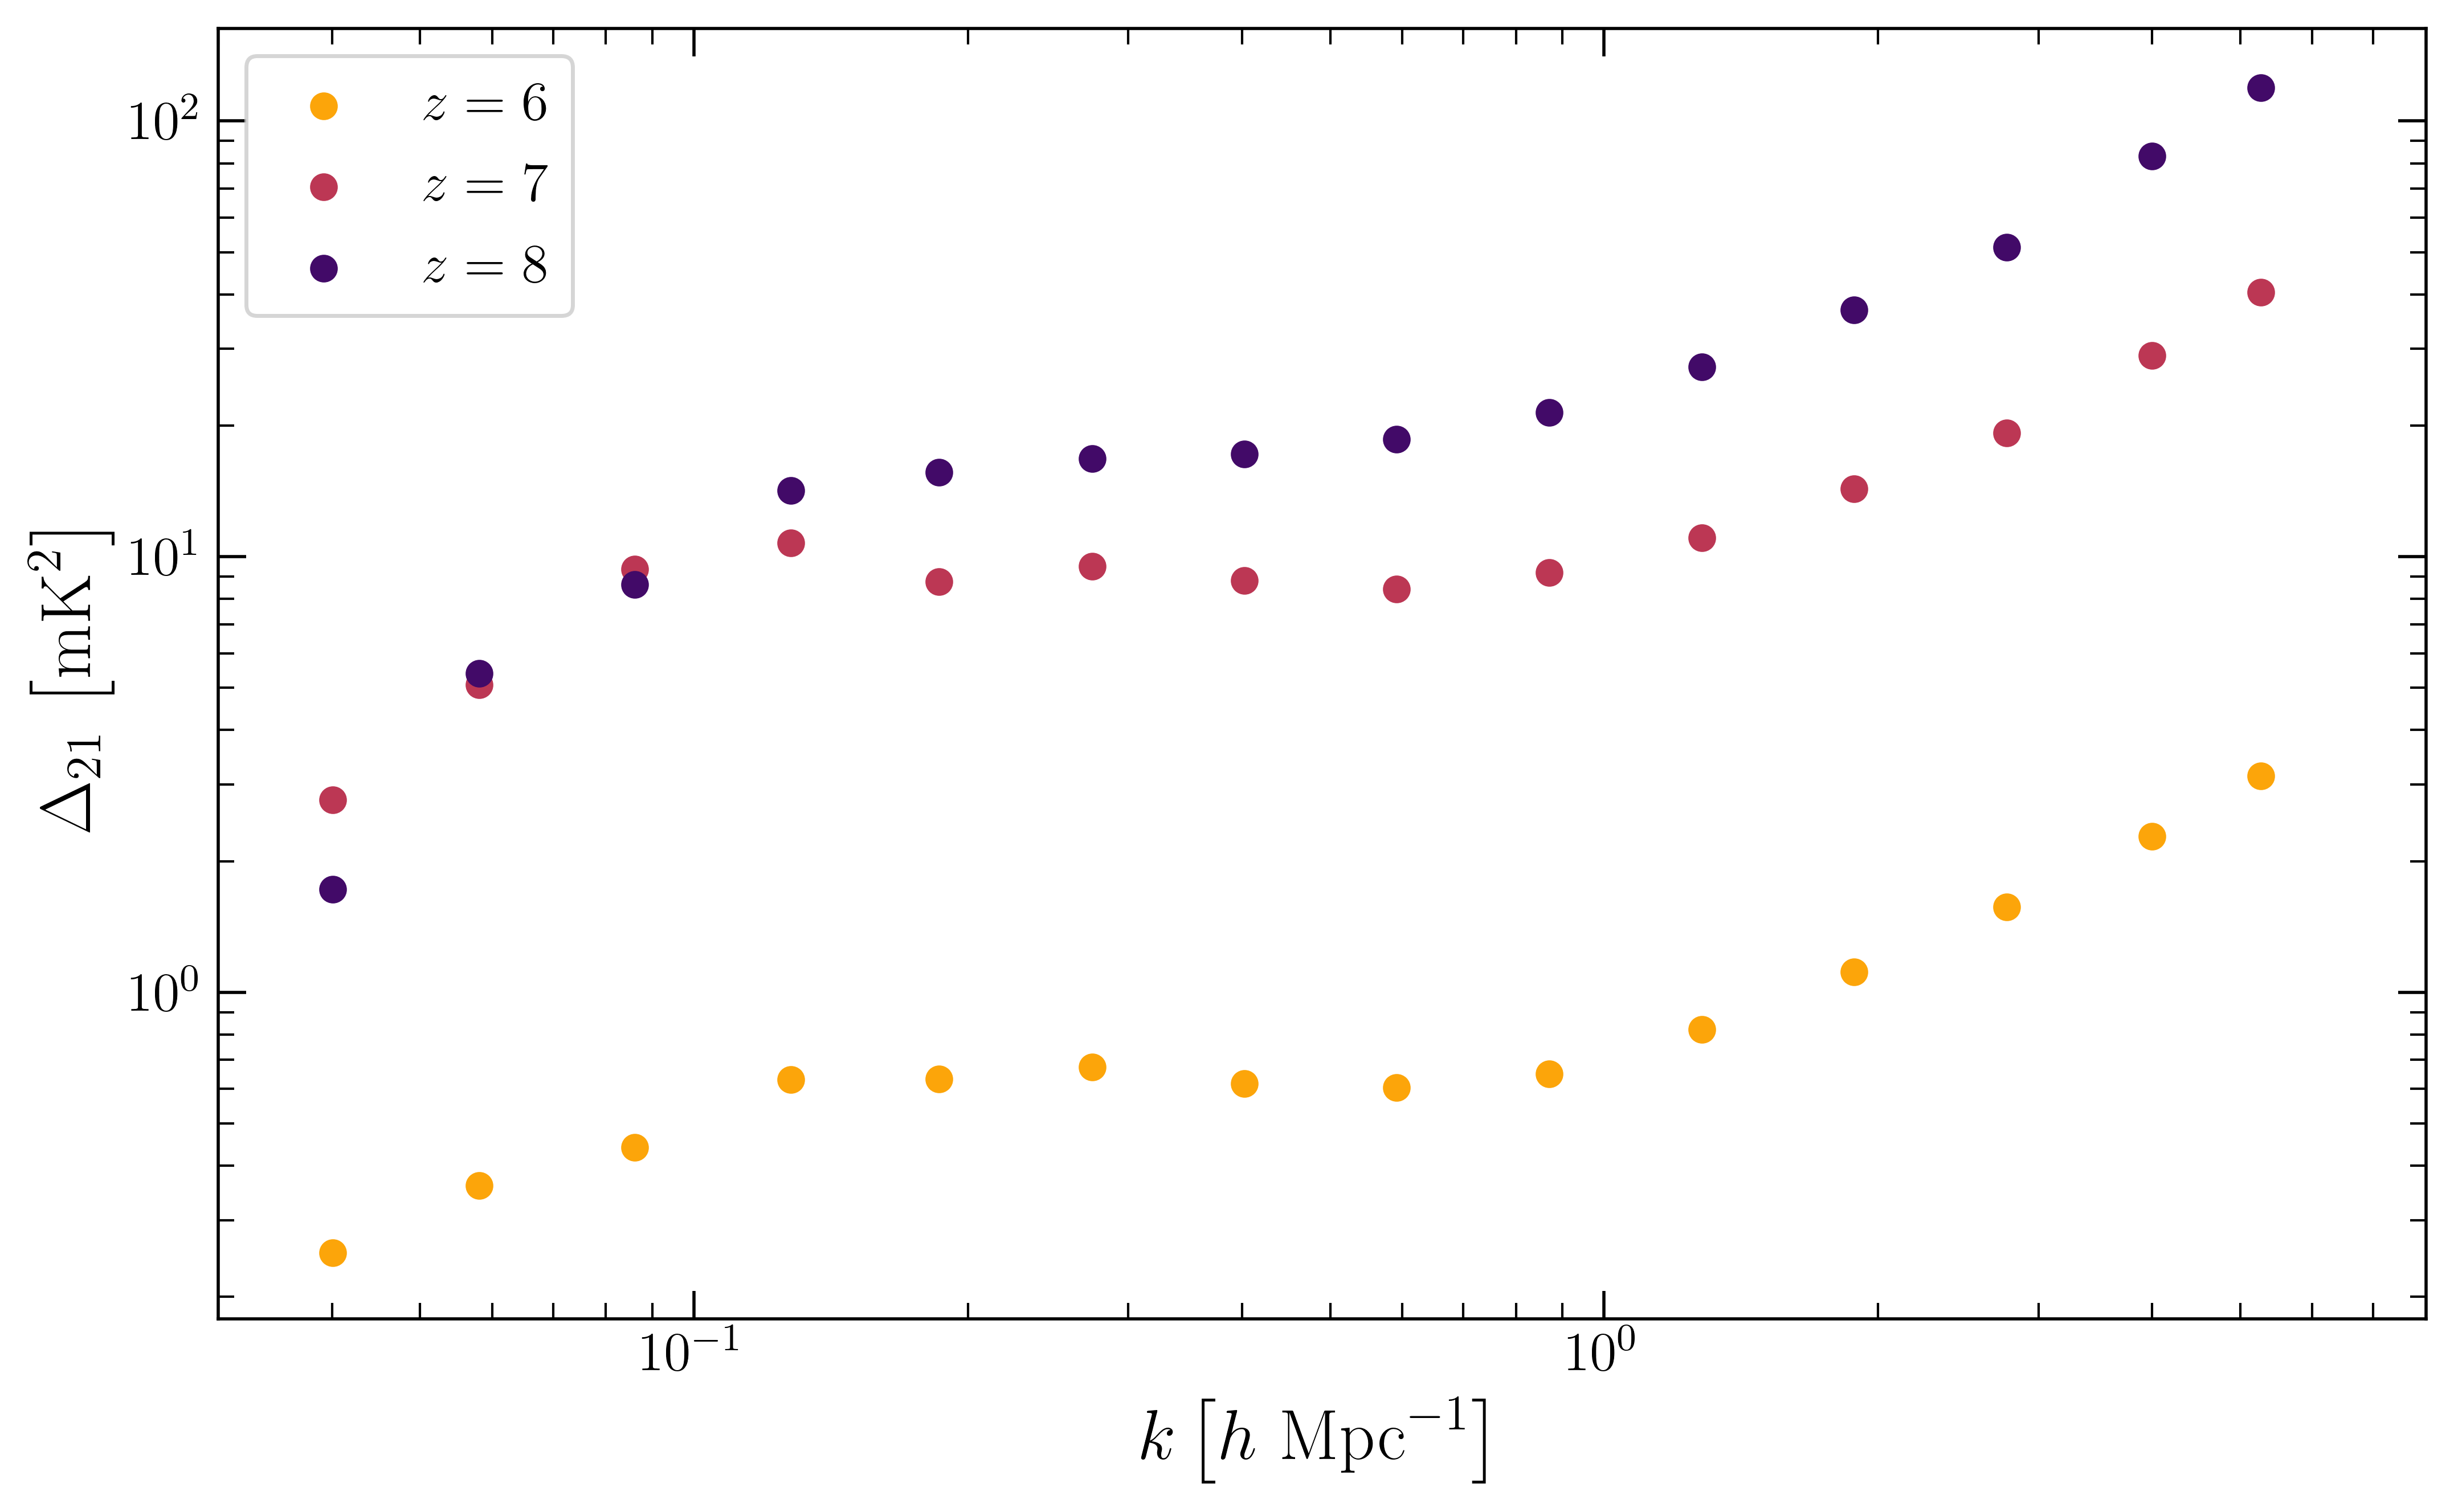
\includegraphics[width=1.\textwidth]{21cm_power_spectrum.png}
	\caption[21\,cm Power Spectrum]{21\,cm power spectra plotted as a function of redshift for the fiducial \fastsim\
           model.}
	\label{fig:21cm_ps}
\end{figure}

The expression above is often referred to as the dimensionless power spectrum.
This can then be used to calculate the dimensional power spectrum by scaling the
dimensionless power spectrum by the mean of the intensity field $\Delta^2_{ij} = \bar{I}_i \bar{I}_j \widetilde{\Delta}^2_{ij}$
These equations can be used to calculate an auto-power spectrum in the case when
$\delta_i$ and $\delta_j$ are the same fluctuation field or a cross-power spectrum
when are they two distinct fields. To calculate the cross-power spectrum, I use
these relationships and the 21\,cm and \lya\ fluctuation fields calculated in the
previous section. The equations for the 21\,cm and \lya\ auto-power spectra and the
21\,cm-\lya\ cross-power spectrum can be seen below.
\begin{align}
    &\Delta^2_{\textrm{Ly} \alpha} \left( k \right) = \left( \nu \bar{I}_{\nu} \right)^2 \widetilde{\Delta}^2_{\textrm{Ly} \alpha} \left( k \right) \\
    &\Delta^2_{21}\left( k \right) = \left(\delta \overline{T}_b \right)^2 \widetilde{\Delta}^2_{21} \left( k \right) \\
    &\Delta^2_{21, \textrm{Ly} \alpha} \left( k \right) = \left(\delta \overline{T}_b \right) \left( \nu \bar{I}_{\nu} \right) \widetilde{\Delta}^2_{21, \textrm{Ly} \alpha} \left( k \right)
\end{align}

\begin{figure}[ht]
	\centering
	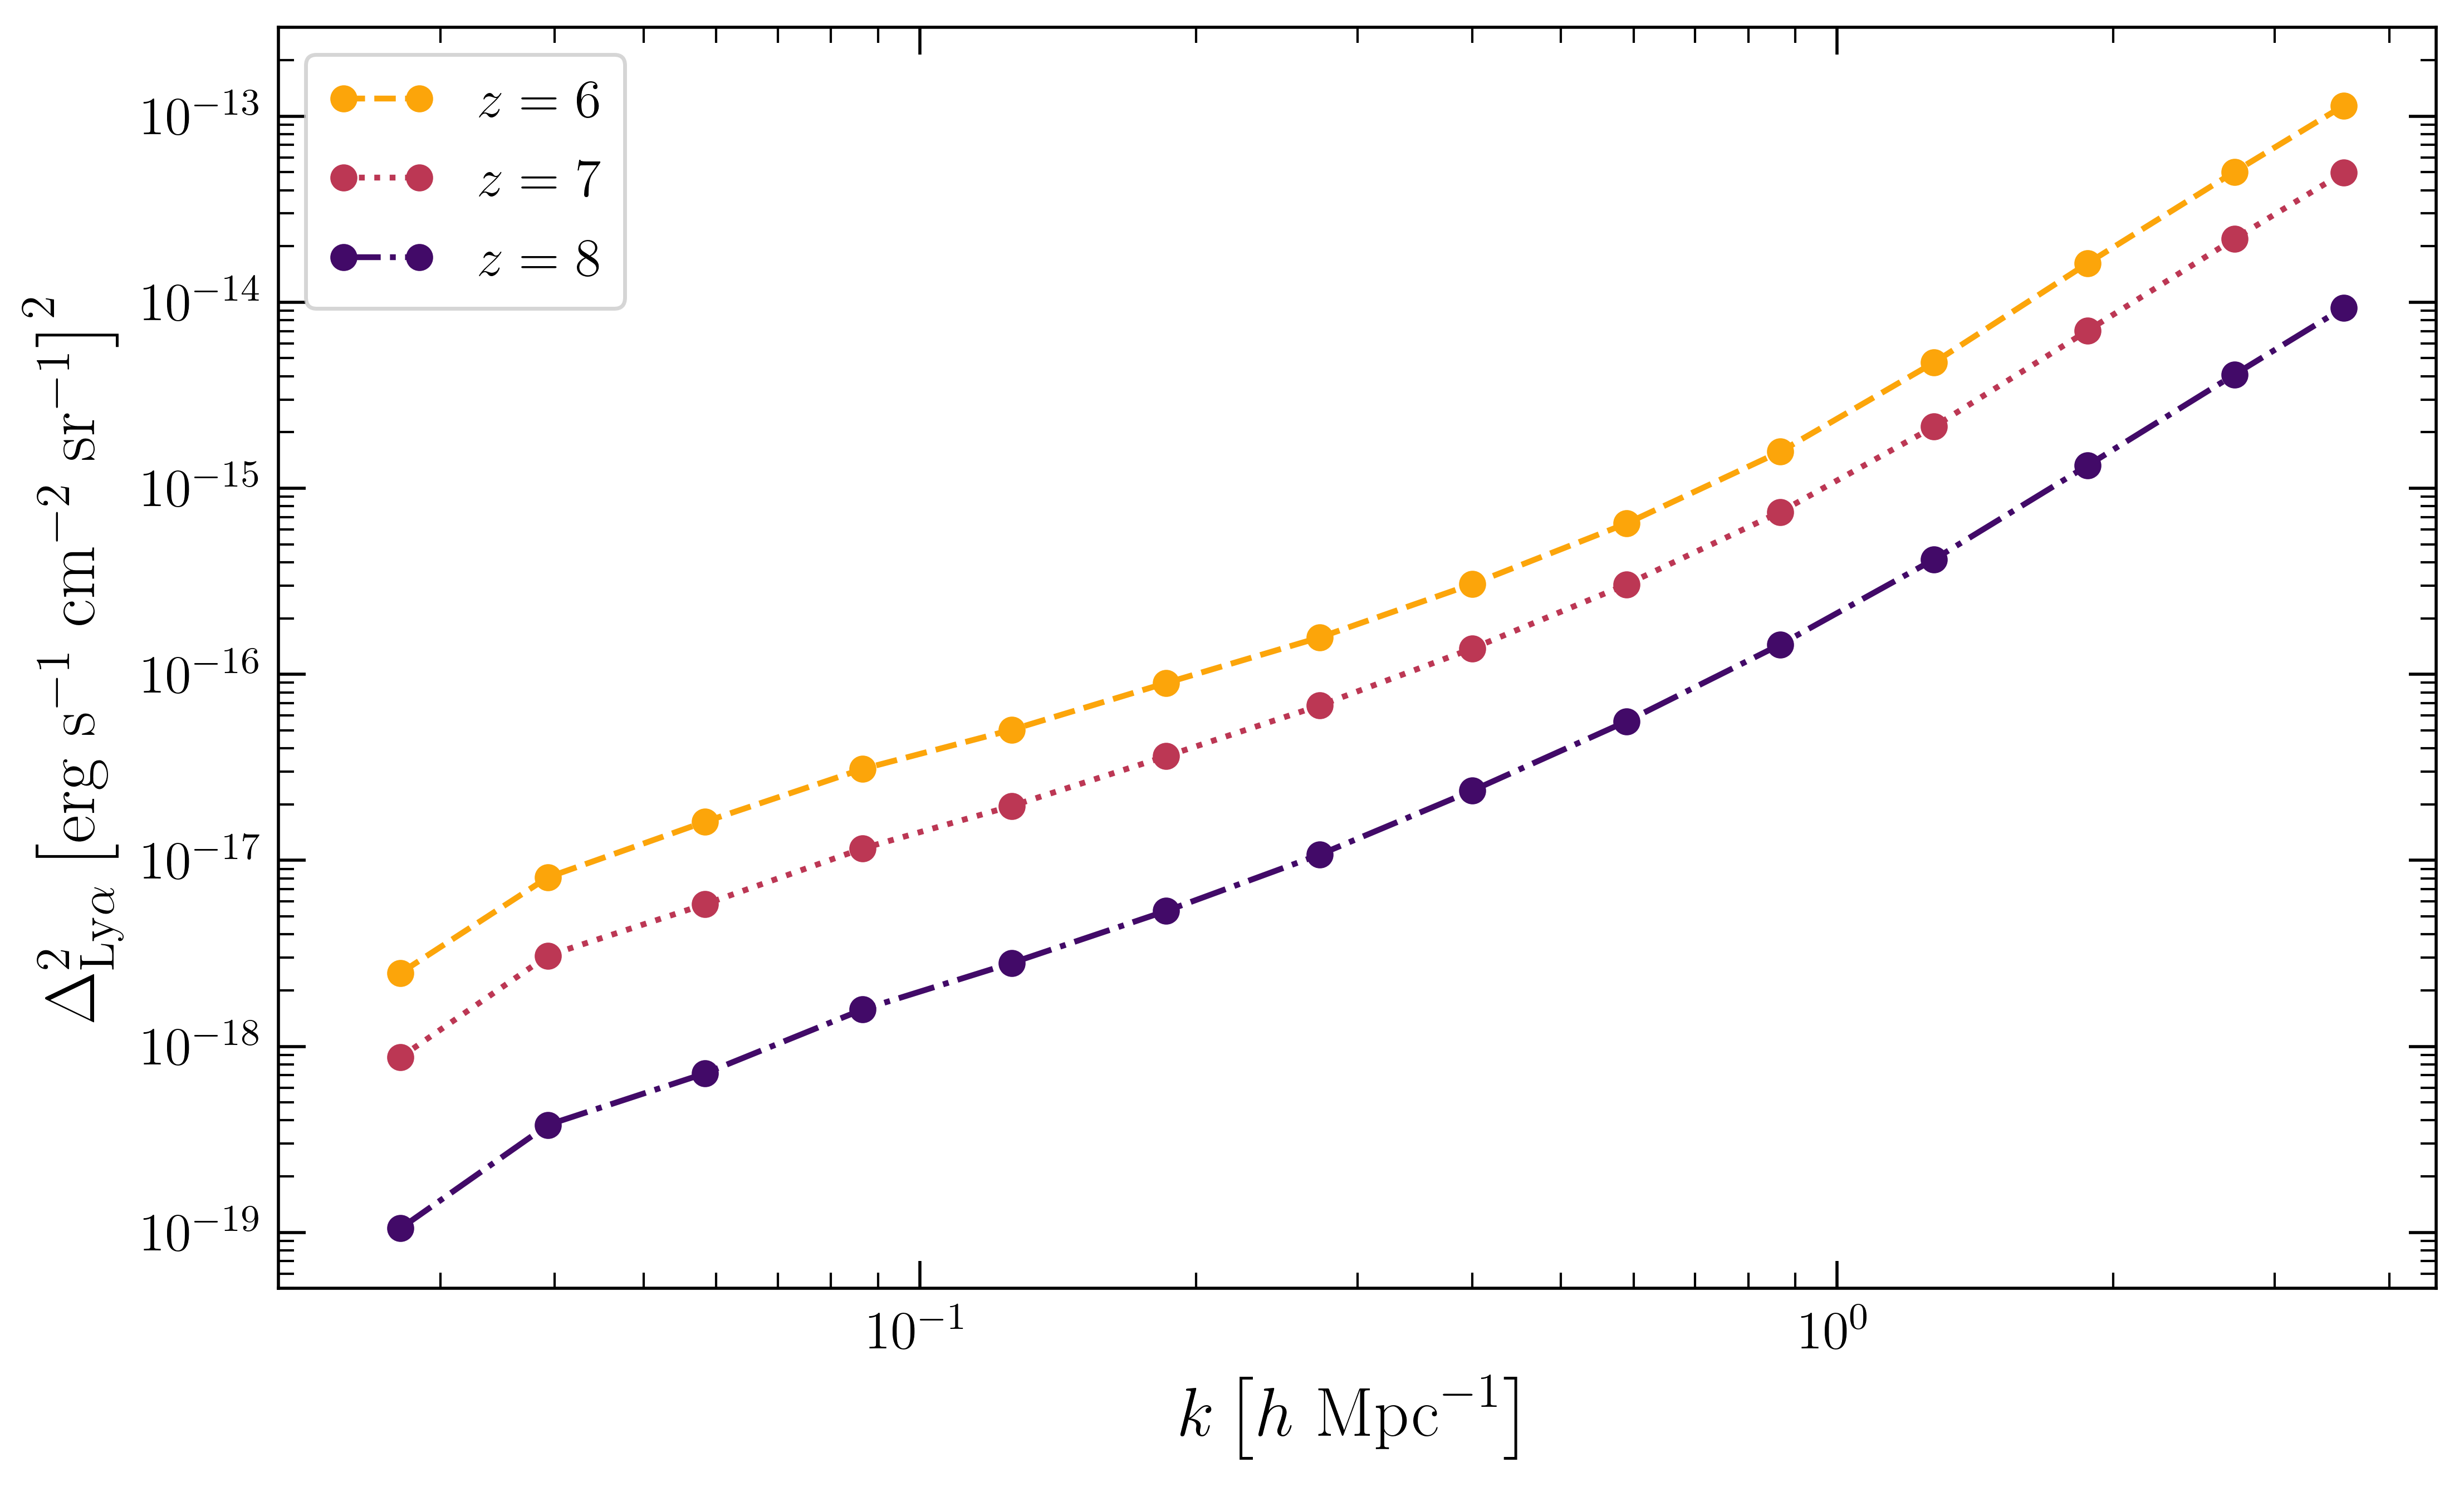
\includegraphics[width=1.\textwidth]{lyman_alpha_pspec.png}
	\caption[\lya\ Power Spectrum]{\lya\ power spectra plotted for the redshift range of interest. Here, I include
           the \lya\ contributions from both LAE's and the ionized IGM.}
	\label{fig:lya_ps}
\end{figure}
It is important to note that when calculating the cross-power spectrum, Planck's
law is used to convert the 21\,cm brightness temperature, $\delta \overline{T}_b$,
to a brightness intensity to simplify the units. The 21\,cm-\lya\ cross-power spectrum
is plotted in Figure \ref{fig:x_ps}. In this figure, it can be seen that the 21\,cm-\lya\
cross-power spectrum turns-over from positive to negative on at each redshifts simulated. This turn-over happens
on the scale of the mean ionized bubble size and increases in scale as reionization
progresses and the bubbles grow.

\begin{figure}[ht]
	\centering
	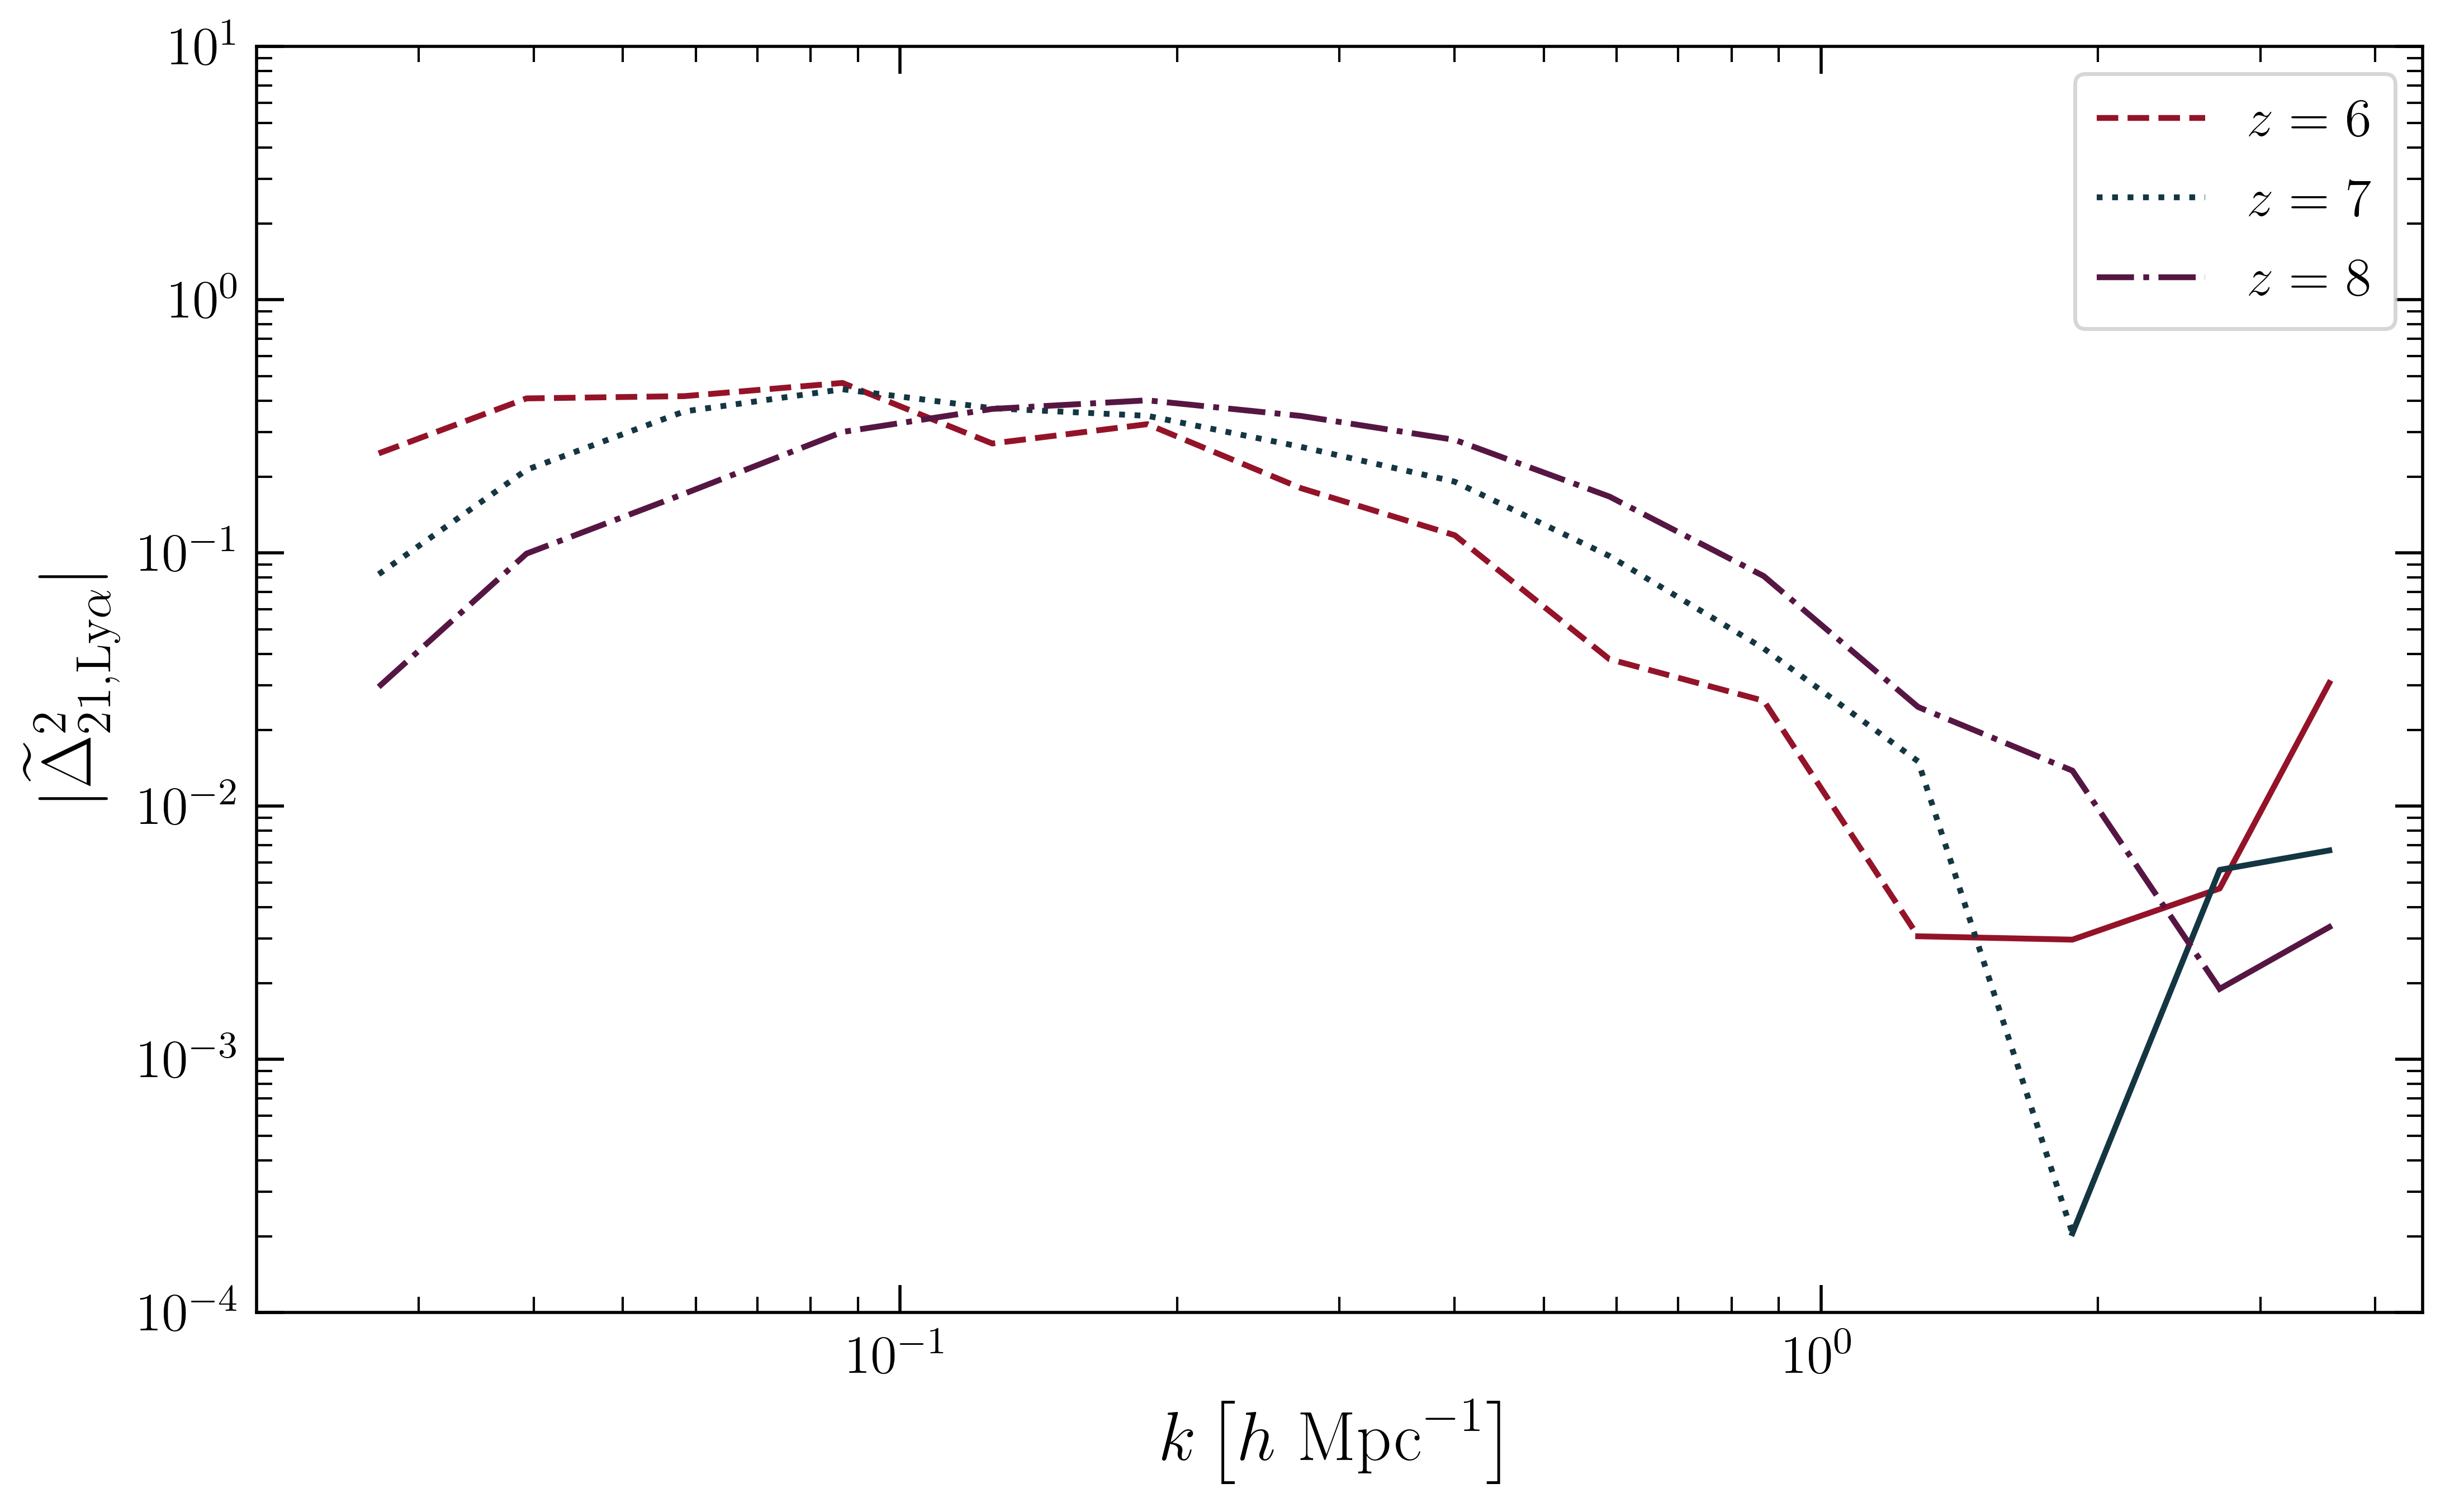
\includegraphics[width=1.\textwidth]{cross_power_spec.png}
	\caption[21\,cm-\lya\ Cross-Power Spectrum]{The dimensionless 21\,cm-\lya\ cross-power spectrum. The
           solid lines on each of the curves represent positive values in the cross-power spectrum, while varying line
           styles on the same curves represent negative values. As expected, the cross-power spectrum turns over from
           positive to negative on the scale of the mean ionized bubble size at that redshift. I also find the cross-power
           spectrum turns over at increasing scales as reionization progresses, tracing the growth of ionized bubbles.}
	\label{fig:x_ps}
\end{figure}

I also use the cross-correlation coefficient as an additional metric of understanding
the IGM at various scales. This expression is defined as,
\begin{equation}
  r \left(k \right) = \frac{\Delta^2_{21, \textrm{Ly} \alpha}\left(k \right)}
                           {\sqrt{\Delta^2_{21} \left(k \right)\Delta^2_{\textrm{Ly} \alpha} \left(k \right)}}.
\end{equation}
This relationship expresses how correlated two fluctuation fields are on different
scales. For correlated modes, $r \left(k \right) > 0$ and for anti-correlated modes
$r \left(k \right) < 0$. As expected, the cross-correlation coefficient for 21\,cm and
\lya\ measurements (shown in Figure \ref{fig:ccc}) transitions from uncorrelated on
small-scales, where the fluctuations from either 21\,cm or \lya\ emission will be found,
to anti-correlated on large-scales, where the fluctuations from the two fields
are not overlapping. It is also interesting to note that the cross-correlation coefficient
progresses from generally anti-correlated at high-redshifts to generally uncorrelated towards
the end of reionization. This change traces the growth of ionized bubbles through
the process of reionization. The scales on which the cross-correlation coefficient
transitions from uncorrelated to anti-correlated represents the size of typical ionized
bubbles around galaxies.

\begin{figure}[ht]
	\centering
	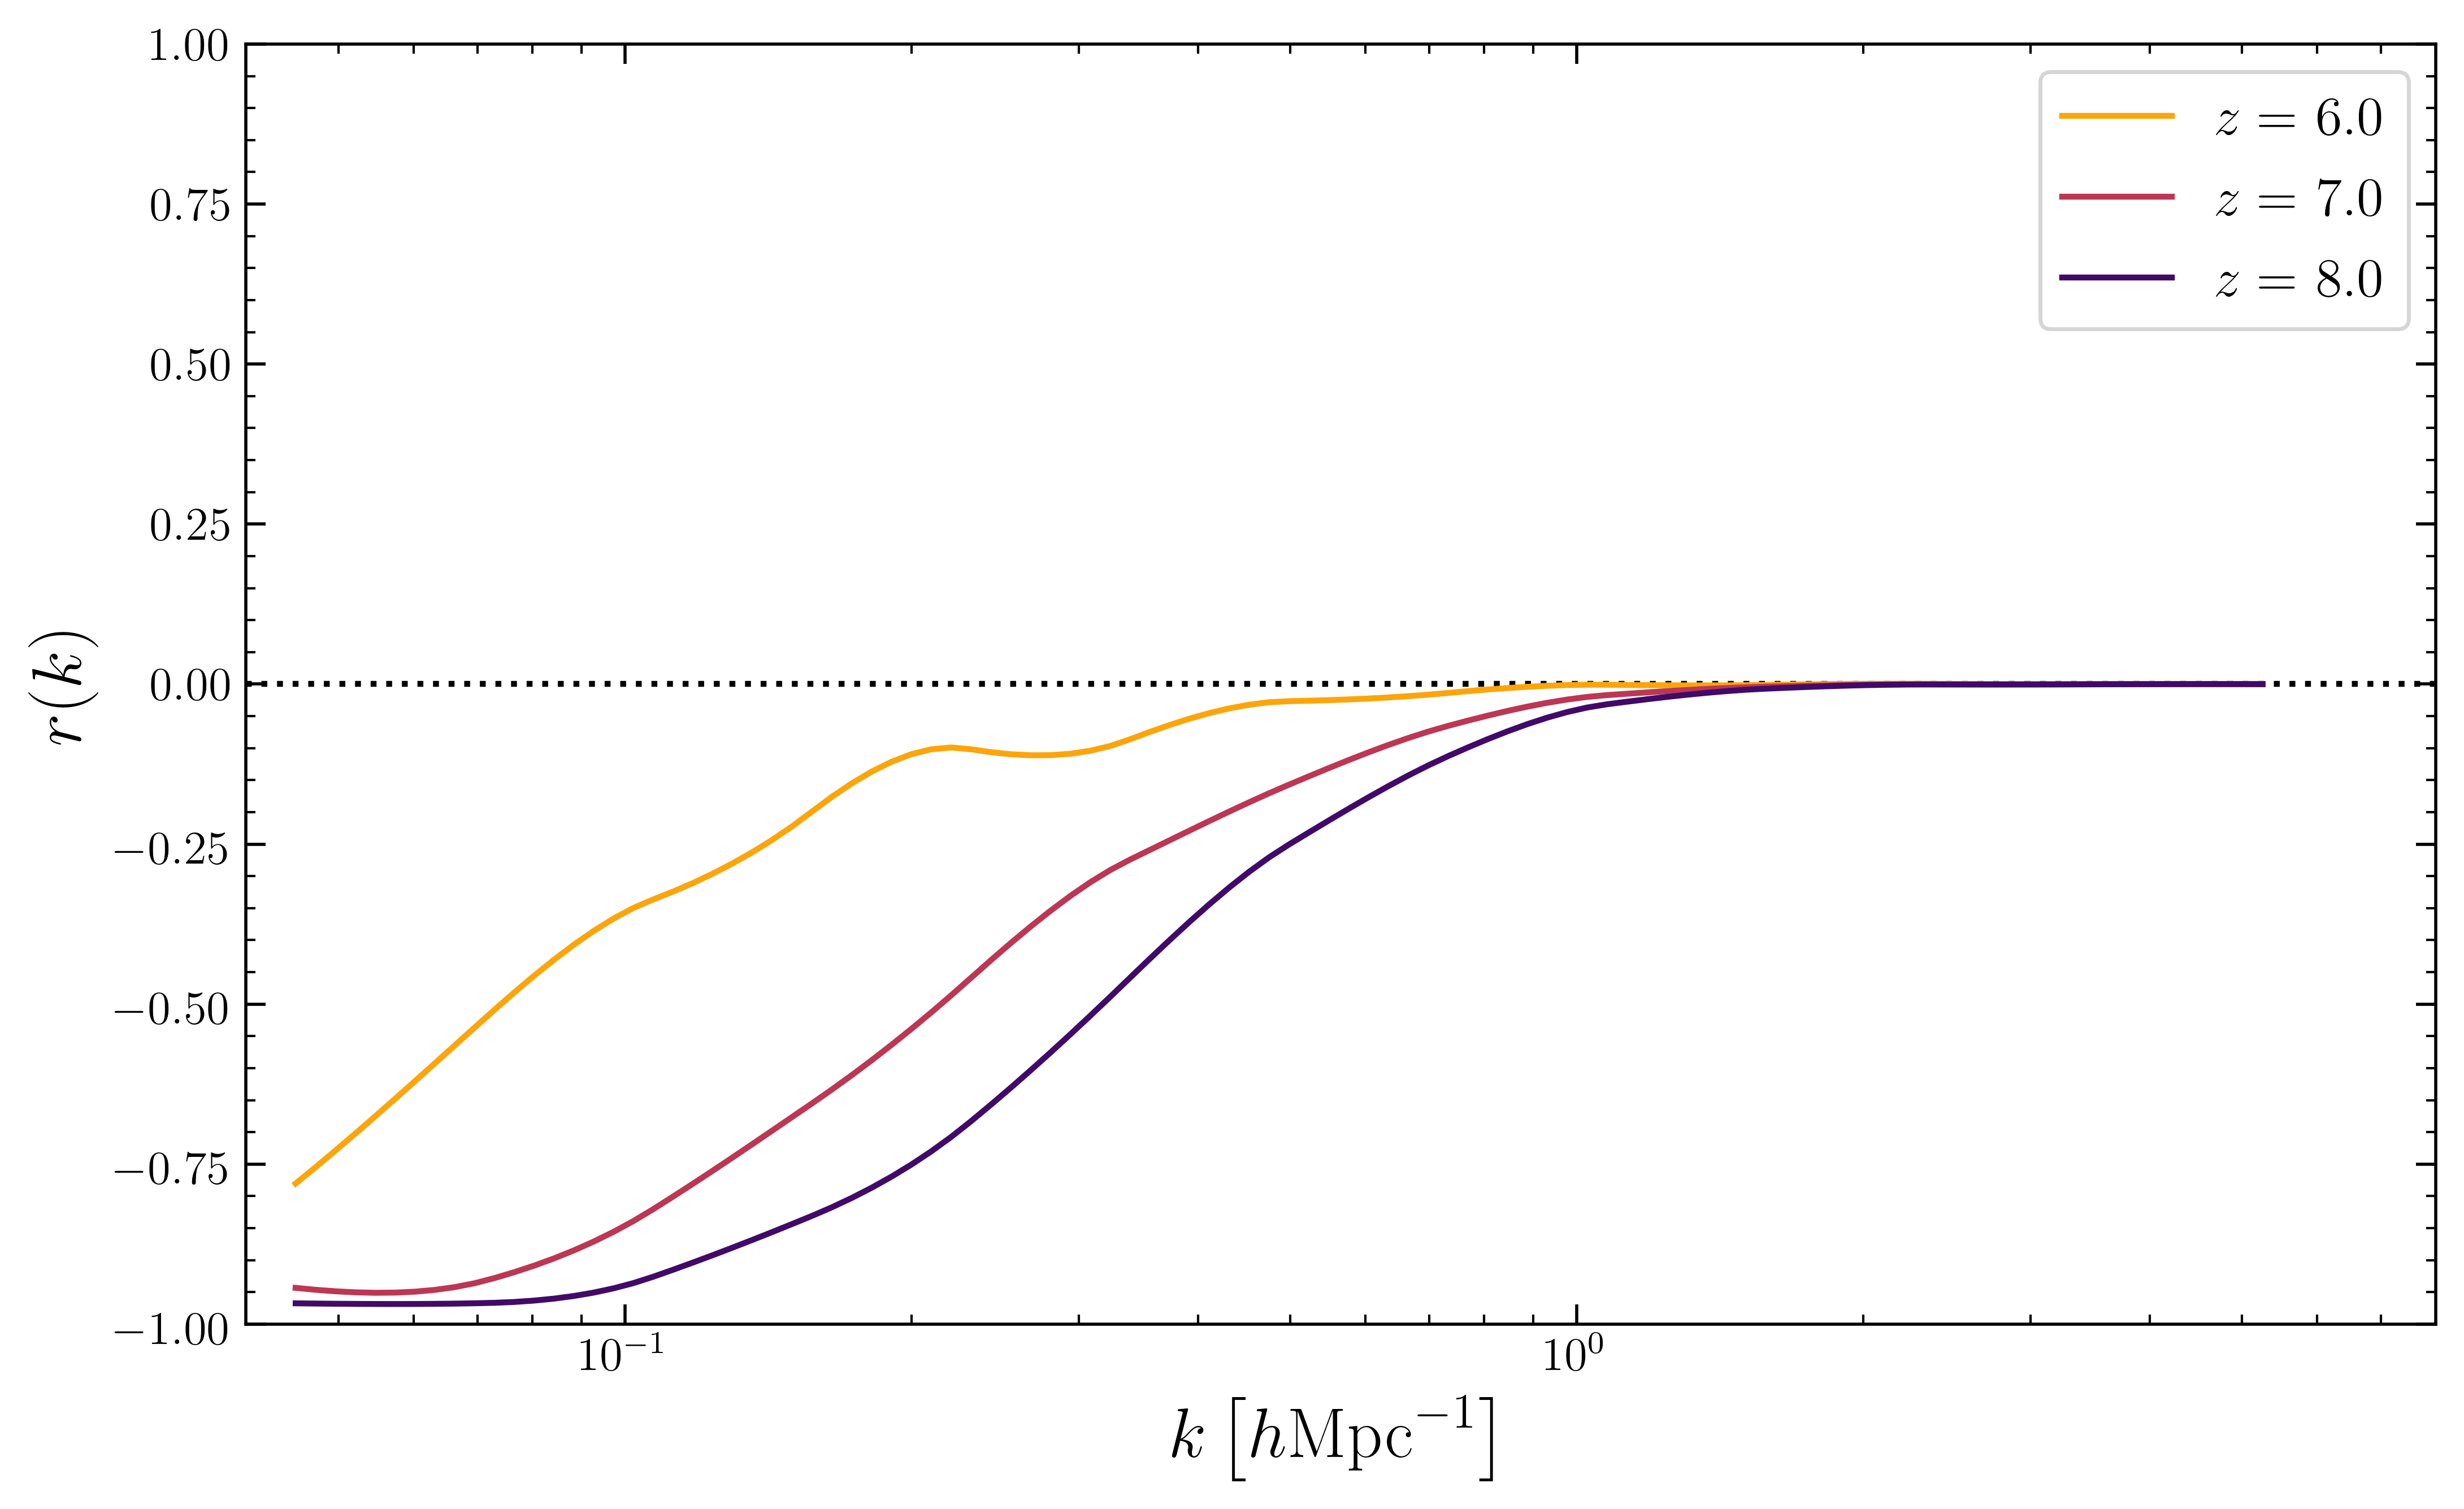
\includegraphics[width=1.\textwidth]{ccc_plot.png}
	\caption[Cross-Correlation Coefficient]{The cross-correlation coefficient (CCC) plotted as a function of scale. Here, a CCC value of
           -1 indicates that emission of 21\,cm and Ly$\alpha$ are completely anti-correlated, while a value of 0 indicates no correlation
           between emission.}
	\label{fig:ccc}
\end{figure}
